%%%%%%%%%%%%%%%%%%%%%%%%%%%%%%%%%%%%%%%%%%%%%%%%%%%%%%%%%%%%%%%%%%%%%
%%                                                                 %%
%% Please do not use \input{\dots} to include other tex files.       %%
%% Submit your LaTeX manuscript as one .tex document.              %%
%%                                                                 %%
%% All additional figures and files should be attached             %%
%% separately and not embedded in the \TeX\ document itself.       %%
%%                                                                 %%
%%%%%%%%%%%%%%%%%%%%%%%%%%%%%%%%%%%%%%%%%%%%%%%%%%%%%%%%%%%%%%%%%%%%%

%%\documentclass[referee,sn-basic]{sn-jnl}% referee option is meant for double line spacing

%%=======================================================%%
%% to print line numbers in the margin use lineno option %%
%%=======================================================%%

%%\documentclass[lineno,sn-basic]{sn-jnl}% Basic Springer Nature Reference Style/Chemistry Reference Style

%%======================================================%%
%% to compile with pdflatex/xelatex use pdflatex option %%
%%======================================================%%

%%\documentclass[pdflatex,sn-basic]{sn-jnl}% Basic Springer Nature Reference Style/Chemistry Reference Style

%%\documentclass[sn-basic]{sn-jnl}% Basic Springer Nature Reference Style/Chemistry Reference Style
\documentclass[sn-mathphys]{sn-jnl}% Math and Physical Sciences Reference Style
%%\documentclass[sn-aps]{sn-jnl}% American Physical Society (APS) Reference Style
%%\documentclass[sn-vancouver]{sn-jnl}% Vancouver Reference Style
%%\documentclass[sn-apa]{sn-jnl}% APA Reference Style
%%\documentclass[sn-chicago]{sn-jnl}% Chicago-based Humanities Reference Style
%%\documentclass[sn-standardnature]{sn-jnl}% Standard Nature Portfolio Reference Style
%%\documentclass[default]{sn-jnl}% Default
%%\documentclass[default,iicol]{sn-jnl}% Default with double column layout

%%%% Standard Packages
%%<additional latex packages if required can be included here>
%%%%

%%%%%=============================================================================%%%%
%%%%  Remarks: This template is provided to aid authors with the preparation
%%%%  of original research articles intended for submission to journals published
%%%%  by Springer Nature. The guidance has been prepared in partnership with
%%%%  production teams to conform to Springer Nature technical requirements.
%%%%  Editorial and presentation requirements differ among journal portfolios and
%%%%  research disciplines. You may find sections in this template are irrelevant
%%%%  to your work and are empowered to omit any such section if allowed by the
%%%%  journal you intend to submit to. The submission guidelines and policies
%%%%  of the journal take precedence. A detailed User Manual is available in the
%%%%  template package for technical guidance.
%%%%%=============================================================================%%%%

\jyear{2023}%

%% as per the requirement new theorem styles can be included as shown below
\theoremstyle{thmstyleone}%
\newtheorem{theorem}{Theorem}%  meant for continuous numbers
%%\newtheorem{theorem}{Theorem}[section]% meant for sectionwise numbers
%% optional argument [theorem] produces theorem numbering sequence instead of independent numbers for Proposition
\newtheorem{proposition}[theorem]{Proposition}%
%%\newtheorem{proposition}{Proposition}% to get separate numbers for theorem and proposition etc.

\theoremstyle{thmstyletwo}%
\newtheorem{example}{Example}%
\newtheorem{remark}{Remark}%

\theoremstyle{thmstylethree}%
\newtheorem{definition}{Definition}%

\raggedbottom
%%\unnumbered% uncomment this for unnumbered level heads




% JAIME: this is to hide font size warnings
\usepackage{anyfontsize}

% JAIME: For 1e-10 notation
\usepackage{siunitx}


\begin{document}

\title[Predicting Audio Features with Last.fm Tags]{Predicting Audio Features with Last.fm Tags}

%%=============================================================%%
%% Prefix	-> \pfx{Dr}
%% GivenName	-> \fnm{Joergen W.}
%% Particle	-> \spfx{van der} -> surname prefix
%% FamilyName	-> \sur{Ploeg}
%% Suffix	-> \sfx{IV}
%% NatureName	-> \tanm{Poet Laureate} -> Title after name
%% Degrees	-> \dgr{MSc, PhD}
%% \author*[1,2]{\pfx{Dr} \fnm{Joergen W.} \spfx{van der} \sur{Ploeg} \sfx{IV} \tanm{Poet Laureate}
%%                 \dgr{MSc, PhD}}\email{iauthor@gmail.com}
%%=============================================================%%

\author*[1]{\fnm{Jaime} \sur{Ramírez Castillo}}\email{Jaime.Ramirez@alu.uclm.es}

\author[1]{\fnm{M. Julia} \sur{Flores}}\email{Julia.Flores@uclm.es}
\equalcont{These authors contributed equally to this work.}


\affil[1]{\orgdiv{Departamento de Sistemas Informáticos}, \orgname{Universidad de Castilla-La Mancha}, \orgaddress{\street{Campus universitario s/n}, \city{Albacete}, \postcode{02071}, \country{Spain}}}


%%==================================%%
%% sample for unstructured abstract %%
%%==================================%%

\abstract{
    In this paper, we discuss a number of experiments to analyze the
    suitability of music label representations to predict certain audio features,
    such as danceability, loudness, or acousticness \dots
}

%%================================%%
%% Sample for structured abstract %%
%%================================%%

% \abstract{\textbf{Purpose:} The abstract serves both as a general introduction to the topic and as a brief, non-technical summary of the main results and their implications. The abstract must not include subheadings (unless expressly permitted in the journal's Instructions to Authors), equations or citations. As a guide the abstract should not exceed 200 words. Most journals do not set a hard limit however authors are advised to check the author instructions for the journal they are submitting to.
%
% \textbf{Methods:} The abstract serves both as a general introduction to the topic and as a brief, non-technical summary of the main results and their implications. The abstract must not include subheadings (unless expressly permitted in the journal's Instructions to Authors), equations or citations. As a guide the abstract should not exceed 200 words. Most journals do not set a hard limit however authors are advised to check the author instructions for the journal they are submitting to.
%
% \textbf{Results:} The abstract serves both as a general introduction to the topic and as a brief, non-technical summary of the main results and their implications. The abstract must not include subheadings (unless expressly permitted in the journal's Instructions to Authors), equations or citations. As a guide the abstract should not exceed 200 words. Most journals do not set a hard limit however authors are advised to check the author instructions for the journal they are submitting to.
%
% \textbf{Conclusion:} The abstract serves both as a general introduction to the topic and as a brief, non-technical summary of the main results and their implications. The abstract must not include subheadings (unless expressly permitted in the journal's Instructions to Authors), equations or citations. As a guide the abstract should not exceed 200 words. Most journals do not set a hard limit however authors are advised to check the author instructions for the journal they are submitting to.}

\keywords{Music information retrieval, Artificial intelligence}

%%\pacs[JEL Classification]{D8, H51}

%%\pacs[MSC Classification]{35A01, 65L10, 65L12, 65L20, 65L70}

\maketitle

\section{Introduction}\label{sec1}

Music information retrieval (MIR) is an interdisciplinary research field that encompasses the extraction,
processing, and knowledge discovery of information contained in music.
MIR research intersects with other fields, such as computer science, signal processing, musicology, and sociology.
The field covers applications in recommendation systems, music classification,
music source separation, and music generation, among others \cite{ramirez2020machine}.

MIR applications often attempt to extract information from the music audio signal,
but analyzing associated metadata is also a common practice.
Audio signals are typically preprocessed and transformed into intermediate formats, such as frequency-based signal representations or hand-crafted audio features.
Associated metadata, such as editorial information, lyrics, or user-generated content is usually in text format.
However, metadata can be available as images of videos, for example, when analyzing album artwork, or music videos.

Depending on the specific MIR application, researchers or practitioners expect different output values.
For example, an application that extracts audio features might return values for the tempo, the key, or the sample rate.
In more complex applications, where, for example, machine learning is used,
applications might return the estimated emotion that a track produces on a listener, or the predicted music genre of a particular track.

Among potentially useful input and output values, research has proved Spotify audio features and Last.fm tags to be significant values to characterize music.
Spotify audio features capture high-level information about the music signal.
Examples of these values are energy, danceability, or valence, among others.
Last.fm tags are text labels that users associate to particular tracks, artists or albums in the Last.fm website.

Both types of values have been used as input values mostly for classification tasks, such as music genre recognition,
where, given Spotify features or Last.fm tasks, the model estimates the music genres of a particular track.
However, these values have not been used as target values by previous research, to the best of our knowledge.
In particular, the focus of this article is on predicting Spotify audio features, given a set of Last.fm tags.

By predicting Spotify audio features, we explore the relationship between subjective perception and concrete musical features.
This approach might help to identify patterns and hidden correlations between how music is percevied, consumed and discovered.

Additionally, predicted audio features could be used in recommendation systems to provide users with explainable recommendations.
Music recommendations,are not always easy to interpret from the perspective of the listener.
Users often get recommendations without meaningful explanations or justifications.
Therefore, by using predicted Spotify features as basis for recommendation, we can explain users why the algorithm suggests a particular track.
This process could be part of an explainable recommendation pipeline, where users enter a set of tags,
and they receive the predicted audio features, the closest tracks to those features, and the distance values between each track and the predicted features.

% The idea is, given a set of tags, to predict a set of audio features that a hypothetic track would exhibit.
% Then, we could build a track selection algorithm that selects actual tracks that are the closest to the predicted audio features.
% This process could be part of an explainable recommendation pipeline, where users enter a set of tags, and they recieve the predicted audio features, the closest tracks to those features, and the distance values between each track and the predicted features.

In the remainder of the article, we explain the data gathering and preparation process, as well as the data input formats and varios models.
We will explore various models for the same track and provide insights on how accurately the prediction can be, by using only Last.fm tags.

\section{Related Research}

In recent years, researchers have studied the use of Last.fm tags in classification and regression tasks.
Several studies have used Last.fm to predict music sentiment or mood.

In the last decade, Last.fm tags have been a popular source of metadata for MIR tasks.
Last.fm tags can contain subjective information the genre, mood, and style of music,
and might be use to characterize certain features of a music piece.


Last.fm tags can be useful when the audio signal available,
for example, due to copyright limitations.

A number of studies have explored the use of Last.fm tags in MIR,
and have shown promising results in predicting various audio features.
% For example, tags such as "acoustic", "live", and "instrumental" have been
% shown to be good predictors of the energy and danceability of a track.
% Similarly, tags such as "happy," "sad," and "angry" have been used
% to predict the valence and arousal of a track.

Researchers have used Last.fm tags.
For example, Laurier et al. analyzed how Last.fm tags categorize mood.
In their study, they created a semantic mood space based on Last.fm tags \cite{laurier2009music}.

For example, {\c{C}}ano and Morisio discuss the process they follow to create a dataset of music
lyrics annotated with Last.fm.
In the creation process, they conclude that Last.fm tags are mostly related to music genre
and positive moods \cite{ccano2017music}.
In a similar direction, Bod{\'o} and Szil{\'a}gyi generated a dataset for lyrics genre classification
by combining the Last.fm with MusicBrainz data \cite{bodo2018connecting}.
MusicBrainz \footnotemark[1] is an online database of music editorial metadata.
\footnote[1]{https://musicbrainz.org/}

The Last.fm data has been the most widely used Last.fm dataset\footnotemark[2] in research.
This dataset is a complementary dataset of the Million Song Dataset (MSD) \cite{Bertin-Mahieux2011}.

\footnotetext[2]{Last.fm dataset, the official song tags and song similarity collection for the Million Song
Dataset, available at: http://millionsongdataset.com/lastfm.}

Spotify, one of the leaders in the music streaming industry...

Additionally, the Spotify audio features have been used in multiple studies.
Historically, these features were also called \emph{Echo Nest audio features}.
Spotify adquired Echo Nest in 2014 and made the audio features available via the Spotify  API
\footnote[3]{https://en.wikipedia.org/wiki/The\_Echo\_Nest}.
Echonest was an online platform that was later acquired by Spotify.
% https://en.wikipedia.org/wiki/The_Echo_Nest

Wang and Horv{\'a}t use audio features to study differences between male and female artists \cite{wang2019gender}


In general, these studies confirm the possibility of extracting knowledge from Last.fm tags.
To the best of our knowledge, no studies have addressed the problem of audio features regression, based solely on Last.fm tags.

Jamdar et al. used EchoNest audio features, combined with lyrics data to classify songs into emotion tags.
These classes were first defined based on a Last.fm tags emotion mapping \cite{jamdar2015emotion}.

Similarly, Non-negative Matrix Factorization was applied in combination with EchoNest audio features
for song recommendations \cite{benzi2016song}.

P4kxspotify is a publicly available dataset that combines music review texts with Spotify audio features.
The dataset creators argue that, although the terms of service prohibits scraping, their work is ethical \cite{pinter2020p4kxspotify}.

In general, Spotify audio features have been used as predictive variables.
We, to the best of our knowledge, are unaware of students that uses these features as target variables.


While Spotify provides a description of the high-level audio features, how they compute or estimate these values is not publicly available.
Panda and Redinho explore the use of Spotify high-level features applied to Music Emotion Recognition (MER) \cite{panda2021does}.
In particular, they identify that the energy, valence, and acousticness values, provided by the Spotify API,
are highly relevant for emotion classification.
They also achieve better performance on MER models by using their own top-100 features, and they determine that,
although these three Spotify features are relevant in terms of characterizing emotion, more features are needed for MER.


% TODO: move explanation to the experiment section.
% \subsubsection{Machine Learning Models}

% Several studies have explored the use of machine learning
% models to predict audio features from audio metadata, such as Last.fm tags.
% % which studies use Last.fm tags as parameters?

% The experiments conduced in this study used two classical regression models,
% Boosted tree regressor and Bayesian ridge regressor.
% These two machine learning models that have been widely used in MIR. % is this true? (refs)

% Boosted tree regressor is a decision tree-based model that sequentially
% adds weak learners to the model to improve its performance.
% Bayesian ridge regressor, on the other hand,
% is a probabilistic model that uses Bayesian inference to estimate
% the parameters of the model.

% Additionally, language models, such as GTP-2 have shown promising results in various
% natural language processing (NLP) and generation.

% In this particular study, GTP-2 has been fine-tuned for regression tasks,
% and has shown good performance in predicting audio features from metadata.

% This paper aims to apply the boosted tree regressor,
%  Bayesian ridge regressor, and GTP-2 models to predict Spotify audio features from Last.fm tags.
% The experiments compare the performance of these models and evaluate their effectiveness
% in predicting various audio features.
% The results of these experiments will provide insights into
% the use of different machine learning models for MIR tasks
% and can have practical applications
% in music recommendation systems and genre or mood recognition.
%
%\textcolor{red}{To be Continued \dots }

\section{Generating a Dataset}


% JAIME
% I have posted a question on the Spotify Developer forum, relative to the release of a dataset
% https://community.spotify.com/t5/Spotify-for-Developers/May-I-publish-an-open-source-dataset-that-contains-Spotify-Audio/td-p/5529259


Before conducting experiments to predict audio features from tags,
we constructed a dataset, by gathering the data from the Last.fm and Spotify APIs.

\subsection{A Single-user Dataset}

This work is scoped within our single-user research area \cite{ramirez2022user}.
In this area, we explore the development of music recommender systems that
characterize the music preferences and listening context only for a single user.
By training our system with single-user data, we also explore the following question: Is it possible to train
recommender systems, and in particular, user-centric systems, by using a single-user dataset?

The user data for this work has been extracted from the
listening history of the corresponding author user in Last.fm
\footnote[4]{https://www.last.fm/user/jimmydj2000}.


Similar to other intelligent systems, recommender systems
must be trained, by using user preference data, to produce
suitable recommendations. For this study,
we leverage the knowledge discovery potential
of large historical listening logs, gathered from Last.fm.

Given the objective of our experiments,
we created a dataset of Last.fm tags and Spotify audio features, indexed by track, by following these steps:



\subsection{Last.fm Tags}

Last.fm is an online music service for users to keep track of their music listening habits.
Last.fm is also an online community where users tag artists, albums, and tracks, according their own taste and perception.

Users apply these tags to
categorize music from their own perspective, which
means that tags do not fit into any structured ontology
or data model.
Tags can refer to any aspect that users consider as a valid descriptor, such as genre,
emotion, or user listenting context.

For nearly two decades, users have been contributing to Last.fm by tagging tracks, albums, and artists with text labels.
Although many of these descriptions are single-worded (e.g \emph{rock}, \emph{dance}, or \emph{happy}),
users can also use short sentences to define a song, such as \emph{I like this track}, or \emph{on the beach}.


\subsubsection{Last.fm Downloaded Data}

Last.fm uses the term \emph{scrobble} to refer to a single track playback,
at a particular moment.
We queried the Last.fm API to download the user{'}s scrobble logs, reported from 2007 to 2022.
For each scrobble, we have gathered the following information:

\begin{itemize}
\item Playback timestamp
\item Track name
\item Artist name
\item Track tags. If the track does not have any tags assigned,
then artist tags have been used
\end{itemize}


For each tag-track mapping, Last.fm includes
a \emph{count} value, which indicates the popularity of the given tag for the track.
Last.fm normalizes this value in the 0-100 range, so the most popular tag for a track can have a
count value of 100.
For example, if \emph{piano} is the most popular tag for a track,
then the track might be probably
associated to the following tuple \verb|(piano, 100)|.

Users normally listen to their favorite tracks several times,
so the amount of unique tracks listened is much smaller
than the number of track plays. In this case, the amount of
individual tracks listened is about 20,000, and the number of scrobblings is, approximately, 90,000.


\subsection{Spotify Audio Features}

After gathering the listening history and track tags from Last.fm, and identifying the unique
tracks that represent the user music collection, we
collected Spotify audio features for each one of those tracks.

The Spotify audio features are numerical values that represent high-level audio information computed from a specific
track. These values characterize a track, musically speaking,
by measuring relevant musical aspects.
For example, a danceability value of 0.95 means
that a particular song is highly suitable for dancing.

The features provided by the Spotify API are listed in
Table \ref{table:spotify-features}.
The reader can find further details about each feature in the Spotify API documentation
\footnote[5]{
      \url{https://developer.spotify.com/documentation/web-api/reference/\#/operations/get-audio-features}
}.


\begin{table}[h!]
      \centering
      \caption{Spotify audio features. These features provide high-level musical information about a track.} \label{table:spotify-features}
      \begin{tabular}{p{0.3\linewidth}p{0.6\linewidth}}
          \toprule
          \bfseries \textbf{Feature name} & \textbf{Description} \\
          \midrule
          \textbf{acousticness} & The track is acoustic. From 0 to 1 \\
          \textbf{danceability} & The track encourages (or is adequate for) dancing. From 0 to 1 \\
          \textbf{duration\_ms}  &  Duration in milliseconds \\
          \textbf{energy}  &  The track is perceived as energetic. From 0 to 1\\
          \textbf{instrumentalness}  &  The track is instrumental. From 0 to 1 \\
          \textbf{key}  &  Key categories encoded as integers. From C (0) to 11 \\
          \textbf{liveness}  &  The audience is audible. From 0 to 1\\
          \textbf{loudness}  &  In decibels. From -60 to 0 \\
          \textbf{mode}  & Major (1) or minor (0) \\
          \textbf{speechiness}  & Does the track contain speeches? From 0 to 1 \\
          \textbf{tempo}  & In beats per minute (BPM) \\
          \textbf{valence} & How happy is the track (BPM). From 0 to 1 \\
          \bottomrule
      \end{tabular}
  \end{table}

The Spotify API failed to provide audio features for a portion of the tracks.
These tracks were filtered out from our experiments.
After filtering tracks that miss Last.fm tags or Spotify audio features,
our dataset contains 14,009 samples.

Considering that the data was gathered from a single user,
we explored the data to verify that the distribution of the Spotify audio features
was comparable to other Spotify datasets.
In particular, we verified that the distribution of the features,
described in Table \ref{table:audio-features-stats} and Figure \ref{fig:audio-features-distribution},
was comparable to the distribution of the \emph{Spotify Audio Features} Kaggle dataset
\footnote[6]{https://www.kaggle.com/datasets/tomigelo/spotify-audio-features}.

\begin{table}[h!]
      \begin{center}
      \begin{minipage}{\textwidth}
      \caption{Audio features description}\label{table:audio-features-stats}%
      \begin{tabular}{@{}lll@{}}
      \toprule
      Feature           & $\mu$ & $\sigma$ \\
      \midrule
      Danceability      & 0.599  & 0.193  \\
      Energy            & 0.631  & 0.233  \\
      Acousticness      & 0.221  & 0.302  \\
      Instrumentalness  & 0.514  & 0.382  \\
      Valence           & 0.435  & 0.279  \\
      \botrule
      \end{tabular}
      \end{minipage}
      \end{center}
\end{table}

\begin{figure}[h!]
      \centering
      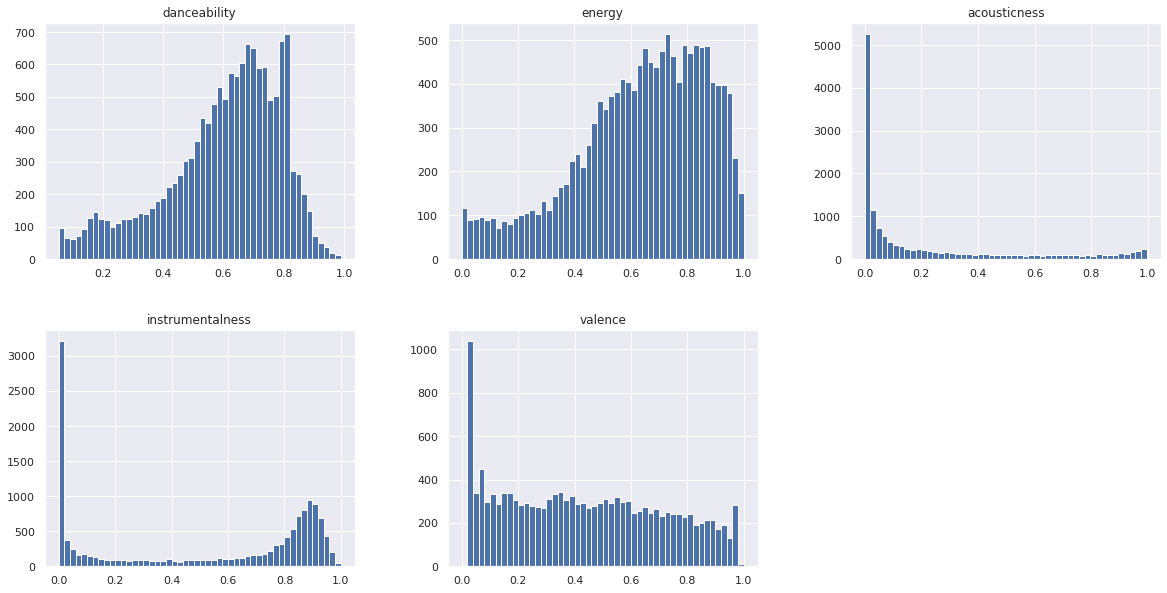
\includegraphics[width=\textwidth]{images/features-distribution.png}
      \caption{Distribution of audio features. These densities are similar to the values shown by the \emph{Spotify Audio Features} Kaggle dataset.}
      \label{fig:audio-features-distribution}
\end{figure}

\subsection{Filtering Missing Values}

Not every track of the approximately unique tracks 20,000 of the Last.fm user{'} listening history
included Last.fm tags and Spotify audio features.
Tracks without Last.fm tags or without Spotify audio features were filtered out.
As a result, of the originally 20,000 tracks included in the listening history,
our dataset final size resulted in 14,009 samples.



\section{Experiments}

We trained commonly used machine learning models to predict an audio feature, given the set of tags for a particular track.

\begin{itemize}
      \item Boosted tree regressor \cite{xgboost}
      \item Naive Bayes Regressor \cite{bayesian}
      \item Fine-tuned GPT-2 model
\end{itemize}

The preceding models require specific input formats.
Therefore, we tested different input formats.

\subsection{Last.fm Tags Input Format}

Each individual sample in the dataset corresponds to a unique track,
and contains the list of Last.fm tag-count tuples (e.g. \verb|[(electronic, 100), (dance, 45), ...]|)
and the values of Spotify audio features.
Before experimenting with machine learning models, we prepared the data in a number of different formats,
each one suitable for specific models.


\subsubsection{Tabular}
With this format, the Last.fm tags are represented as a table.
Each tag is defined by a column and each cell contains the count value of a tag for a track.
A cell is 0 if a tag is missing for a track.

The number of columns is limited to the top-K tags.
Counting the total amount of Last.fm tags in the user collection resulted, initially, in more than five million tags.
We quickly confirmed that building a tabular data set, in which every row contains millions of columns (Last.fm tags)
was doable, but presented scalability problems.
Therefore, we reduced the number of tags by picking a subset of the most relevant tags.

The reduction algorithm is simple: calculate a weighted sum of all the tags appearances and pick the top 1000.
The sum is weighted be- cause we use the count attribute.
This attribute is present in every Last.fm track-tag association and provides a measure of the strength of a particular tag in a specific track.
Note that this reduction is an initial approach, which, similar to other phases, can be extended or improved in the future. For this particular case, dimensionality reduction algorithms, such as PCA, are good candidates for forthcoming iterations of this work.

The input data passed is formatted in tabular format, as follows:

\begin{itemize}
      \item Given that $Tags_{k}$ is the set of most $k$ frequent Last.fm tags in the user listening history
            and, where each $tag \in Tags_{k}$.
      \item Given that $Audio$ is the set of Spotify audio features, where each $feat \in Audio$.
      \item For each $track$:
      \begin{itemize}
            \item $X_{track},_{tag}$ is the strengh of $tag$ for $track$. This value is in the $0-100$ range.
            \item $y_{track},_{feature}$ is the value of the audio feature $y$ for $track$.
      \end{itemize}
\end{itemize}

An example of this data format is provided in table \ref{tabular_tags_format}.

\begin{table}[h]
      \begin{center}
      \begin{minipage}{\textwidth}
      \caption{Tabular data format for Last.fm tags in XGBoost and Bayesian regressors}\label{tabular_tags_format}%
      \begin{tabular}{@{}lllllll@{}}
      \toprule
      Track                         & $X_{electronic}$ & $X_{ambient}$ & $X_{\dots}$ & $y_{energy}$ & $y_{valence}$ & $y_{\dots}$ \\
      \midrule
      Massive Attack - Blue Lines   & 62               & 6             &  \dots      & 0.496        & 0.947         & \dots  \\
      The Beta Band - Squares       & 40               & 3             &  \dots      & 0.446        & 0.507         & \dots  \\
      \dots                         & \dots            & \dots         &  \dots      & \dots        & \dots         & \dots  \\
      \botrule
      \end{tabular}
      \end{minipage}
      \end{center}
\end{table}

When generating training data by track, the tabular formats present sparsity problems.

For tabular representations, we need to defined a fixed set of columns as tags.
For most of tracks, most columns are 0.

The sparsity of a matrix is the number of zero-valued elements divided by the total number of elements
(e.g., m * n for an m * n matrix) is called the sparsity of the matrix.


\subsubsection{Tabular Tokens}

Tags are converted to text tokens. Columns represent token positions, and cells contain the token at a particular position, for a track.
To tokenize tags, we have used the GTP2 tokenizer.
Because the tokenizer requires a string as input, we have converted the set of tags for each track into a string.
To \emph{stringify} the tags, we have concatenated tags with multiple strategies:

\begin{itemize}
      \item By including tag popularity: `rock 2, pop 1`.
      \item By repeating tags based on popularity: `rock rock, pop`.
      \item By ordering by popularity: `rock, pop`.
\end{itemize}


In this particular case, the $X$ values of the tabular input data are tokens.
These tokens are obtained from passing the a string of concatenated Last.fm tags through a tokenizer.
The formal definition of this data format is as follows:

\begin{itemize}
      \item Given that $X_l$ is the token vocabulary, where $l$ is the maximum vocabulary length.
      \item Given that $Audio$ is the set of Spotify audio features, where each $feat \in Audio$.
      \item For each $track$:
      \begin{itemize}
            \item $X_{track},_{n}$ is token found at position $n$, after tokenizing the tags string.
            \item $y_{track},_{feature}$ is the value of the audio feature $y$ for $track$.
      \end{itemize}
\end{itemize}

An example of this data format is provided in table \ref{tabular_token_format}.

\begin{table}[h]
      \begin{center}
      \begin{minipage}{\textwidth}
      \caption{Tabular data format for tokens in XGBoost and Bayesian regressors}\label{tabular_token_format}%
      \begin{tabular}{@{}llllllll@{}}
      \toprule
      Track                         & $X_{0}$ & $X_{1}$ & $X_{2}$ & $X_{\dots}$ & $y_{energy}$ & $y_{valence}$ & $y_{\dots}$ \\
      \midrule
      Massive Attack - Blue Lines   & 101     & 5099    & 6154    &  \dots      & 0.496        & 0.947         &  \dots  \\
      The Beta Band - Squares       & 101     & 4522    & 2600    &  \dots      & 0.446        & 0.507         &  \dots  \\
      \dots                         & \dots   & \dots   & \dots   &  \dots      & \dots        & \dots         &  \dots  \\
      \botrule
      \end{tabular}
      \end{minipage}
      \end{center}
\end{table}


\subsection{Text}

When using transformer models, the input data is a string.
We must represent the Last.fm tags, which are initially in the $(tag name, tag popularity)$ form, to a a string.

After converting to a string, the formal definition of the input data is as follows:

\begin{itemize}
      \item Given that $X$ is tags represented as text.
      \item Given that $Audio$ is the set of Spotify audio features, where each $feat \in Audio$.
      \item For each $track$:
      \begin{itemize}
            \item $X_{track},_{n}$ is set of tags for $track$, encoded as a single string.
            \item $y_{track},_{feature}$ is the value of the audio feature $y$ for $track$.
      \end{itemize}
\end{itemize}

An example of this data format is provided in table \ref{text_format}.

\begin{table}[h]
      \begin{center}
      \begin{minipage}{\textwidth}
      \caption{Text data format for tokens in XGBoost and Bayesian regressors}\label{text_format}%
      \begin{tabular}{@{}lllll@{}}
      \toprule
      Track                         & $X$                                   & $y_{energy}$ & $y_{valence}$ & $y_{\dots}$ \\
      \midrule
      Massive Attack - Blue Lines   & "hip hop, chill, bristol, \dots"      & 0.496        & 0.947         & \dots  \\
      The Beta Band - Squares       & "alternative rock, folk, \dots"       & 0.446        & 0.507         & \dots \\
      \dots                         & \dots                                 & \dots        & \dots         & \dots  \\
      \botrule
      \end{tabular}
      \end{minipage}
      \end{center}
\end{table}




\subsection{Boosted Tree Regressor}

We configured the boosted tree regressor model with the training parameters listed in table \ref{table_xgboost_training_params}.

\begin{table}[h]
      \begin{center}
      \begin{minipage}{174pt}
      \caption{Training parameters for XGBoost regressor}\label{table_xgboost_training_params}%
      \begin{tabular}{@{}llll@{}}
      \toprule
      Parameter               & Value \\
      \midrule
      objective               & reg:squarederror  \\
      base score              & 0.5 \\
      booster                 & gbtree  \\
      colsample bylevel       & 1 \\
      colsample bynode        & 1 \\
      colsample bytree        & 1 \\
      gamma\footnotemark[1]   & 0 \\
      learning rate           & 0.300000012 \\
      max delta step          & 0 \\
      max depth               & 6 \\
      min child weight        & 1 \\
      estimators              & 200  \\
      n jobs                  & 12  \\
      num parallel tree       & 1 \\
      predictor               & auto  \\
      random state            & 0 \\
      reg alpha               & 0 \\
      reg lambda              & 1 \\
      scale pos weight        & 1 \\
      subsample               & 2 \\
      tree method             & auto  \\
      \botrule
      \end{tabular}
      \footnotetext[1]{Minimum loss reduction required to make a further partition on a leaf node of the tree.}
      \end{minipage}
      \end{center}
\end{table}


\subsection{Naive Bayes Regressor}

The Naive Bayes Regressor, and in particular, Bayesian Ridge, is the model used for regression in this case.

% COMMENT copied FROM BayesianRidge source code
% https://github.com/scikit-learn/scikit-learn/blob/9aaed4987/sklearn/linear_model/_bayes.py#L24
%
%     There exist several strategies to perform Bayesian ridge regression. This
%     implementation is based on the algorithm described in Appendix A of
%     (Tipping, 2001) where updates of the regularization parameters are done as
%     suggested in (MacKay, 1992). Note that according to A New
%     View of Automatic Relevance Determination (Wipf and Nagarajan, 2008) these
%     update rules do not guarantee that the marginal likelihood is increasing
%     between two consecutive iterations of the optimization.

The training parameters are listed in table \ref{table_bayesian_training_params}.

\begin{table}[h]
      \begin{center}
      \begin{minipage}{174pt}
      \caption{Training parameters for XGBoost regressor}\label{table_bayesian_training_params}%
      \begin{tabular}{@{}llll@{}}
      \toprule
      Parameter                     & Value \\
      \midrule
      Maximum iterations            & 300   \\
      Tolerance\footnotemark[1]     & \num{1e-03} \\
      alpha 1                       & \num{1e-06} \\
      alpha 2                       & \num{1e-06} \\
      lambda 1                      & \num{1e-06} \\
      lambda 2                      & \num{1e-06} \\
      \botrule
      \end{tabular}
      \footnotetext[1]{Tolerance for the stopping criteria.}
      \end{minipage}
      \end{center}
\end{table}


\subsection{Fine-tuned Transformer}

Transformers are a type of neural network architecture that has been widely used in natural language processing (NLP) tasks,
such as text generation and question answering.
They were first introduced in 2017 by paper [REF: "Attention Is All You Need"]
and have become one of the most popular models due to their ability
to handle long-range dependencies and process variable-length inputs.

One popular variant of transformers is the Generative Pre-trained Transformer 2 (GPT-2),
which was introduced by OpenAI in 2019.
GPT-2 is a language model that has been trained on a large corpus of text,
and can generate coherent and fluent text that resembles human-written language.
GPT-2 has achieved remarkable results in a wide range of natural language processing tasks, including text generation, machine translation, and question answering.

In this study, we have used GPT-2 as a regressor to predict Spotify audio features from Last.fm tags. The basic idea behind this approach is to feed a string of concatenated Last.fm tags as input to the GPT-2 model, and then use the model's output as the predicted value of a specific Spotify audio feature. By training the GPT-2 model on a large dataset of Last.fm tags and corresponding Spotify audio features, 
we aim to learn the complex relationships between these two types of data and to use this knowledge to evaluate the prediction accuracy of Spotify audio features based on Last.fm tags.

To train the GPT-2 model as a regressor, we used a supervised learning approach.
Specifically, we collected a large dataset of Last.fm tags and corresponding Spotify audio features, and used this dataset to train the GPT-2 model to predict Spotify audio features from Last.fm tags. We used a mean squared error loss function to optimize the model's performance during training, and we also employed techniques such as early stopping and learning rate scheduling to prevent overfitting and improve generalization performance.
\textcolor{red}{Under development...}

\subsection{Experiments Execution and Results}

Table \ref{table:experiment_results} summaries the experiment results.
The table provides RMSE values for each experiment.


\begin{table}[h!]
      \begin{center}
      \begin{minipage}{\textwidth}
      \caption{Experiment results. Cells values correspond to the RMSE value.}\label{table:experiment_results}%
      \begin{tabular}{@{}lllllll@{}}
      \toprule
      M         & Input format                        & Danceab...       & Acoustic...    & Energy    & Valence    & Instrumen... \\
      \midrule
      Base      &                                     & 0.276            & 0.438           & 0.329     & 0.395      & 0.541          \\
      Bayes     & 100 tags\footnotemark[1]            & 0.159            & 0.261           & 0.197     & 0.243      & 0.307          \\
      Tree      & 100 tags                            & 0.154            & 0.257           & 0.188     & 0.240      & 0.302          \\
      Bayes     & 1000 tags                           & 0.153            & 0.253           & 0.190     & 0.237      & 0.299          \\
      Tree      & 1000 tags                           & 0.149            & 0.249           & 0.184     & 0.236      & 0.291          \\
      Bayes     & 10000 tags                          & 0.152            & 0.251           & 0.189     & 0.236      & 0.297          \\
      Tree      & 10000 tags                          & 0.148            & 0.250           & 0.181     & 0.236      & 0.290          \\
      Bayes     & 100 tokens D\footnotemark[2]        & 0.307            & 0.307           & 0.238     & 0.281      & 0.383          \\
      Tree      & 100 tokens D                        & 0.274            & 0.274           & 0.212     & 0.256      & 0.330          \\
      Bayes     & 1000 tokens D                       & 0.201            & 0.315           & 0.249     & 0.248      & 0.399          \\
      Tree      & 1000 tokens D                       & 0.173            & 0.278           & 0.215     & 0.220      & 0.339          \\
      Bayes     & 10000 tokens D                      & 0.359            & 0.507           & 0.394     & 0.479      & 0.613          \\
      Tree      & 10000 tokens D                      & 0.172            & 0.276           & 0.217     & 0.266      & 0.342          \\
      Bayes     & 100 tokens O\footnotemark[3]        & 0.191            & 0.305           & 0.237     & 0.282      & 0.376          \\
      Tree      & 100 tokens O                        & 0.179            & 0.294           & 0.225     & 0.271      & 0.350          \\
      Bayes     & 1000 tokens O                       & 0.237            & 0.343           & 0.276     & 0.339      & 0.428          \\
      Tree      & 1000 tokens O                       & 0.182            & 0.294           & 0.224     & 0.270      & 0.353          \\
      Bayes     & 10000 tokens O                      & 0.237            & 0.343           & 0.276     & 0.339      & 0.428          \\
      Tree      & 10000 tokens O                      & 0.182            & 0.294           & 0.225     & 0.267      & 0.353          \\
      Bayes     & 100 tokens TC\footnotemark[4]       & 0.191            & 0.304           & 0.236     & 0.281      & 0.380          \\
      Tree      & 100 tokens TC                       & 0.172            & 0.280           & 0.211     & 0.262      & 0.342          \\
      Bayes     & 1000 tokens TC                      & 0.202            & 0.320           & 0.247     & 0.248      & 0.404          \\
      Tree      & 1000 tokens TC                      & 0.174            & 0.282           & 0.215     & 0.220      & 0.344          \\
      Bayes     & 10000 tokens TC                     & 0.234            & 0.341           & 0.274     & 0.321      & 0.430          \\
      Tree      & 10000 tokens TC                     & 0.175            & 0.281           & 0.214     & 0.270      & 0.345          \\
      .....     & .............                       & .....            & .....           & .....     & .....      & .....          \\
      GPT       & Duplicated\footnotemark[2]          & 0.157            & ...             & ...       & ...        & ...            \\
      GPT       & Ordered\footnotemark[3]             & 0.149            & ...             & ...       & ...        & ...            \\
      GPT       & Tags,Counts\footnotemark[4]         & \textbf{0.145}   & ...             & ...       & ...        & ...            \\
      \botrule
      \end{tabular}
      \footnotetext[1]{Tags in tabular format. Given $(rock, 3)$, the cell in the $rock$ column contains \verb*|3|.}
      \footnotetext[2]{Duplicated tokens in tabular format. Tags $(rock, 3), (pop, 2)$, are converted to the \verb*|"rock, rock, rock, pop, pop"| string, 
      which a tokenizer converts to the list of input tokens (e.g. \verb*|[101,1005,16588,1005,2531, ...]|).
      These tokens are passed to the model in tabular format. Columns are $token_1$, $token_2$, $...$, $token_N$.}
      \footnotetext[3]{Ordered tokens in tabular format. Tags $(rock, 3), (pop, 2)$, are converted to the \verb*|"rock, pop"| string,
      which a tokenizer converts to the list of input tokens (e.g. \verb*|[101,1005,16588,1005,2531, ...]|).
      These tokens are passed to the model in tabular format. Columns are $token_1$, $token_2$, $...$, $token_N$.}
      \footnotetext[4]{Tokens in tabular format from tags and counts. Tags $(rock, 3), (pop, 2)$, are converted to the \verb*|"'rock' 3, 'pop' 2"| string,
      which a tokenizer converts to the list of input tokens (e.g. \verb*|[101,1005,16588,1005,2531, ...]|).
      These tokens are passed to the model in tabular format. Columns are $token_1$, $token_2$, $...$, $token_N$.}
      \footnotetext[2]{String. Given tags $(rock, 3), (pop, 2)$, input is formatted as \verb*|"rock, rock, rock, pop, pop"|.}
      \footnotetext[3]{String. Given tags $(rock, 3), (pop, 2)$, input is formatted as \verb*|"rock, pop"|.}
      \footnotetext[4]{String. Given tags $(rock, 3), (pop, 2)$, input is formatted as \verb*|"'rock' 3, 'pop' 2"|.}
      \end{minipage}
      \end{center}
\end{table}

\subsubsection{Results for Tabular Data Models}

\begin{figure}[h!]
      \centering
      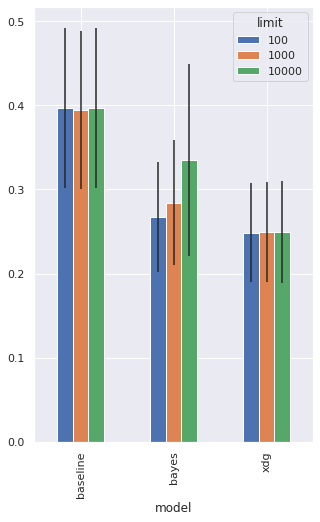
\includegraphics[width=0.5\textwidth]{images/rmse_by_model_and_limit.png}
      \caption{RMSE mean and standard deviation by model and tags/tokens limit.}
      \label{fig:rmse_by_model_and_limit}
\end{figure}


\begin{figure}[h!]
      \centering
      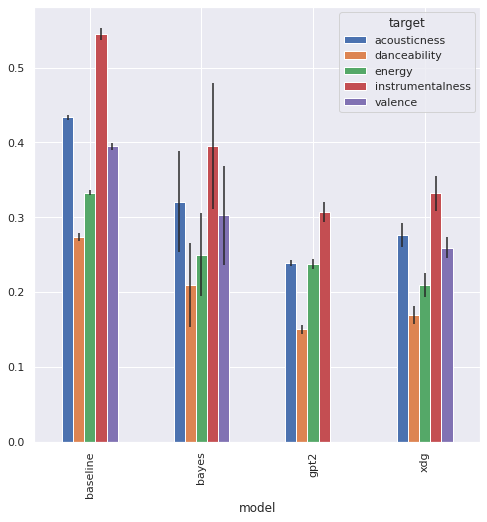
\includegraphics[width=0.7\textwidth]{images/rmse_by_model_and_feature.png}
      \caption{RMSE mean and standard deviation by model and audio feature.}
      \label{fig:rmse_by_model_and_feature}
\end{figure}


\begin{figure}[h!]
      \centering
      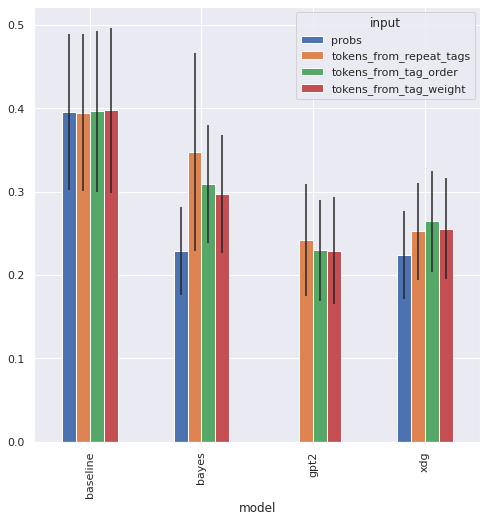
\includegraphics[width=0.7\textwidth]{images/rmse_by_model_and_input.png}
      \caption{RMSE mean and standard deviation by model and input type (tag probablities or tokens).}
      \label{fig:rmse_by_model_and_input}
\end{figure}


\begin{figure}[h!]
      \centering
      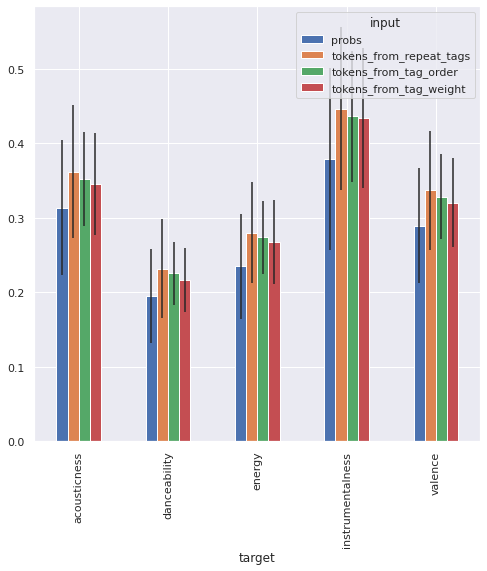
\includegraphics[width=0.7\textwidth]{images/rmse_by_feature_and_input.png}
      \caption{RMSE mean and standard deviation by audio feature and input type (tag probablities or tokens).}
      \label{fig:rmse_by_feature_and_input}
\end{figure}

\section{Conclusions}

In general, we believe that this novel approach that has the potential to benefit both listeners and researchers.
By combining subjective user-generated tags with objective audio features,
we can gain new insights into the complex relationship between perception and audio signal in music.

Our approach also presents limitations.
One limitation is the assumption of a strong relationship between Last.fm tags and Spotify features, which may not be true in all cases.
Future work could explore other sources of input values, possibly related to the user context, to improve the accuracy of the predictions.



\textcolor{red}{TODO}


\section{Acknowledgments}

\textcolor{red}{TODO}



%%===========================================================================================%%
%% If you are submitting to one of the Nature Portfolio journals, using the eJP submission   %%
%% system, please include the references within the manuscript file itself. You may do this  %%
%% by copying the reference list from your .bbl file, paste it into the main manuscript .tex %%
%% file, and delete the associated \verb+\bibliography+ commands.                            %%
%%===========================================================================================%%

\bibliography{bibliography}% common bib file
%% if required, the content of .bbl file can be included here once bbl is generated
%%\input sn-article.bbl

%% Default %%
%%\input sn-sample-bib.tex%

\end{document}
